\documentclass{IEEEtran}

\usepackage{graphicx,tikz}
%\usepackage{fullpage}
\usepackage{amsthm}
\usepackage{amssymb}
\usepackage{amsmath}
%\usepackage{algorithm}
%\usepackage{algorithmicx}
%\usepackage{algpseudocode}
%\usepackage{booktabs}
%\usepackage{color}

%\renewcommand{\baselinestretch}{0.95}
%\setlength{\textfloatsep}{0.1cm}
%\setlength{\abovecaptionskip}{0.1cm}

\begin{document}

\title{\Large\bf Privacy Preserving Metric-based Ranked Search over Encrypted Cloud Data}
\author{Shiyu Ji\\ shiyu@cs.ucsb.edu}
\date{}
\maketitle

\newtheorem{definition}{Definition}
\theoremstyle{definition}
\newtheorem{theorem}{Theorem}
\theoremstyle{plain}
\newtheorem{lemma}{Lemma}
\theoremstyle{plain}
\newtheorem{corollary}{Corollary}
\theoremstyle{plain}

\section{Introduction}

With the advance of cloud computing and information retrieval, secure search over encrypted cloud data has attracted extensive research interest \cite{WC12,Cao14,Sun13,WYL14,SLH14,SLL15,LLD15,WSL15,Xia16}. Most of the state-of-art research works focus on keyword relevance based search \cite{WC12,WYL14,LLD15,SLL15,WSL15}, or similarity based search \cite{Cao14,Sun13,SLH14,Xia16}. The measure of relevance or similarity is usually fixed, e.g., TF $\times$ IDF rule \cite{WC12} or cosine similarity \cite{Cao14,Xia16}, etc. It is still very open how to securely search over encrypted cloud data and rank the resulted documents based on various network metrics, e.g., PageRank \cite{PR99}, SimRank \cite{JW02}, Betweenness Centrality \cite{Bran01}, Jaccard Index \cite{Jac89}, etc. This paper attempts to give such a secure search framework supporting metric-based ranking.

We summarize our major contributions as follows:
\begin{enumerate}
\item We are the first to propose a privacy preserving scheme for all metric-based ranked search over encrypted cloud data.
\end{enumerate}

\section{Problem Formulation}
\subsection{The System and Threat Model}

\begin{figure}
\centering
\includegraphics[width=0.8\linewidth]{system_model.eps}
\caption{The architecture of ranked similarity search over encrypted cloud data.}
\label{fig:system_model}
\end{figure}

As in Fig. \ref{fig:system_model}, we consider a cloud data hosting service which consists of three entities: the data owner, the data users and the semi-trusted cloud data server. The data owner has a collection of documents that need to be outsourced to the semi-trusted cloud server. The outsourced documents must be encrypted since the data owner does not want to reveal the documents to the semi-trusted server. The encryption scheme will be given later. On the other hand, the data users would like to search over the encrypted documents. To enable this, the data owner prepares a search index of the outsourced documents, and then uploads the encrypted index to the server. On a keyword-based search request, an authorized data user firstly gets the corresponding trapdoors and keys from the data owner, and uses the keys to generate the query given the keyword, and then sends the search query to the cloud server. Upon receiving the search query, the server should securely search on the index (i.e., without revealing any information about the documents), and return the tags of top $k$ document (with highest scores based on some network metric) to the user. Finally the user uses the returned tags to securely obtain the documents from the cloud server, who should not know which documents are obtained. That is, the access pattern should be hidden.

We assume the cloud server is \emph{semi-trusted}, or \emph{honest-but-curious}, i.e., the server will honestly do as described above, but it also wants to know any information of the outsourced documents and the submitted search queries. We consider the \emph{Ciphertext-Only Attack}, in which the server only has the submitted encrypted documents and queries, but it initially has no knowledge about their plaintext. We will also consider another stronger attack, in which we assume the server has some knowledge about the outsourced content, e.g., the frequency distribution. Thus some statistical attacks may be launched.

\subsection{Our Goals}
We want to design an efficient and secure ranked search scheme over encrypted cloud data that satisfies the requirements above, and we also want it to keep privacy to some extent.

\textbf{Efficiency}. The algorithms should be efficient, including: 1) encryption over the documents and index, 2) search over the encrypted index, 3) securely fetch the document given its tag, etc.

\textbf{Dynamic updating support}. The data owner should be able to update the documents and index efficiently at any time, e.g., insertion and deletion.

\textbf{Confidentiality}. The content of the documents, the entries (not yet queried) in the index and the queried keywords should not be revealed to the cloud server. We allow the cloud server to know the queried entries in the index since we would like to delegate the metric computation to the server for efficiency. Usually the computation will use the data in the queried entries.

\textbf{Privacy preserving}. We want to prevent the cloud server from learning anything about the outsourced documents, the keywords queried by users, or document access pattern. We will investigate the cases as follows:
\begin{itemize}
\item \textbf{Document privacy}. The server should not learn any information about the outsourced documents, e.g., which document was returned to the user.
\item \textbf{Keyword privacy}. The server should not be able to know any information about the keywords in the search queries.
\item \textbf{Oblivious document access}. The characteristic of document access pattern should not be learned by the cloud server. This can be achieved by using blind storage \cite{NPG14}.
\end{itemize}

\subsection{Notations and Definitions}
\label{sec:prelim}
\begin{itemize}
\item $F$ \---- The collection of the documents to be outsourced: $F = \{f_1, \cdots, f_n\}$ where $f_i$ denotes the $i$-th document in plaintext. Each document $f_i$ contains several keywords $w_{i,1}$, $w_{i,2}$, etc.
\item $C$ \---- The collection of the encrypted documents in $F$: $C = \{c_1, \cdots, c_n\}$ where each $c_i$ is the ciphertext of document $f_i$.
\item $W$ \---- The collection of all the keywords contained in the document $F$: $W = \{w_1, w_2, \cdots, w_m\}$ where $w_i$ denotes the $i$-th keyword.
\item $I$ \---- The index built for the keywords $W$, where each index entry is a list containing information about the tags of documents $C$.
\item $r$ \---- The search request $r$, which contains the keywords which are interesting to the user.
\item $q$ \---- The query vector determined by the keywords in the search request $r$.
\item $T$ \---- The tags of top $k$ documents: $T = \{\tau_1, \tau_2, \cdots, \tau_k\}$ with the highest scores based on the query $q$.
\item $V[i]$ \---- The $i$-th component of the vector $V$. For example, if $V = (0,1,2)^T$, then $V[1] = 0$, $V[2] = 1$ and $V[3] = 2$.
\end{itemize}

\emph{Inverted Index} is a popular technique in information retrieval \cite{TAOCPv1}. An inverted index consists of multiple inverted lists, each of which corresponds to one keyword, i.e., each list of keyword $w_i$ contains all the documents that contain the keyword $w_i$. Also the entries in the lists can include more information, such as the location of the document, the positions of the keyword within the document, etc. Inverted index outperforms most of other solutions when searching over very large volume of documents.

\emph{Graph model} is one of the standard ways to define a network \cite{NM10}. Usually the relations among the outsourced documents give a network, e.g., the citations, the references, etc. Many graph model based metrics have been proposed to evaluate the importance and centrality of each vertex in the network, e.g., PageRank, Betweenness Centrality, SimRank, Clustering Coefficient, etc. Most modern search engines rank the search results based on some network metric since users are often interested in the most keyword-related documents.

\emph{Blind storage} \cite{NPG14} is an efficient oblivious transfer (OT) protocol implementation under the honest-but-curious adversary model. The locations of the stored documents are distributed independently from each other in the view of the cloud server. The cloud server will return the queried document correctly without knowing which one is returned. The communication and storage overhead of blind storage is moderate.


\section{Basic Secure Ranked Search Scheme}
In this section we propose our secure ranked search scheme, assuming the data owner can compute the metric scores of the documents before outsourcing them to the cloud server.

\newcommand{\Enc}{\textsf{Enc}}
\subsection{The Basic Scheme}
The data owner randomly samples the symmetric encryption keys $k, k'$ (given a security parameter $\lambda$) and chooses a pseudorandom function $f$. Let $\Enc$ denote the symmetric encryption and let $H(\cdot)$ be the collision resistant hash function. 
\begin{itemize}
\item {\bf Setup}: Given the document tags $T$ and the keywords $W$, the data owner constructs the inverted index $I$. Denote by $F_{w_i}$ the documents containing $w_i$ and denote by $T_{w_i}$ the tags of documents $F_{w_i}$. The data owner computes the metric scores of the documents in $F_{w_i}$ and sort their tags $T_{w_i}$ in descending order. The index $I$ takes the keywords in $W$ as keys, and takes the sorted $T_{w_i}$ as the posting list of keyword $w_i$. 
\item {\bf IndexBuild}: The data owner replaces each key $w_i$ in the inverted index $I$ by its hash value $H(w_i)$, and replaces its associated list $T_{w_i}$ by the encryption $\Enc(T_{w_i}||r)$ under the key $f_k(w_i)$ (the value of $f$ on input $w_i$ under the key $k$), where $||$ denotes concatenation, and $r$ is a random binary string that is used to hide the length information of $T_{w_i}$. Then the data owner outsources all the encrypted documents $\Enc_{k'}(F)$ and the encrypted inverted index $I$ to the cloud server. The encrypted documents should be stored into a blind storage from the cloud server.
\item {\bf Retrieval}: Suppose the user would like to query the keyword $w_j$. With some help from the data owner, the user is able to compute $H(w_j)$ and $f_k(w_j)$. Then the user sends the tuple $(H(w_j), f_k(w_j))$ to the cloud server. Upon receiving the query, the server can locate the list by using $H(w_j)$ and decrypt the corresponding list $\Enc(T_{w_j}||r)$ by using $f_k(w_j)$. Then by restoring $T_{w_j}$ in the list, the server will return the first $K$ tags in $T_{w_j}$ to the user.
\item {\bf OT}: Upon receiving the $K$ top tags, the user communicates with the blind storage of the cloud server and safely obtains the corresponding $K$ documents.
\end{itemize}

\subsection{Security Analysis}
\textbf{Confidentiality} of the documents and index entries (not yet queried) is guaranteed by symmetric encryption (e.g., 256-bit AES with CBC mode), which makes sure that it is computationally infeasible to distinguish its ciphertext from truly random strings.

\textbf{Document privacy} is protected by the blind storage, which assures that the cloud server has no idea which encrypted document was returned to the user. 

\textbf{Keyword privacy} is protected by the collision resistant hash function $H(\cdot)$ and the pseudorandom function $f$, i.e., given $H(w_i)$ and $f_k(w_i)$ (the adversary has no idea on the key $k$), it is computationally infeasible to find the keyword $w_i$.

\textbf{Oblivious document access} is guaranteed by the blind storage scheme.

\subsection{Discussions}
One drawback of the basic scheme is that it requires the data owner to pre-compute the metric scores of all the documents, which may be quite time-consuming. A natural idea is to delegate the computation to the cloud server, and the scores should be computed \emph{only} when the lists are queried.

Also the basic scheme has to re-compute the metric scores and re-encrypt the corresponding lists when inserting or deleting documents. In our next improved scheme, this can be done more efficiently.


\section{Delegating Secure Ranked Search Scheme}
In this section we propose our improved scheme that allows the data owner to safely delegate the metric computation to the cloud server. Our scheme can also allow the data owner to dynamically insert and delete documents to the cloud server efficiently.

\subsection{The Delegating Scheme}
Same as before, the data owner randomly samples the symmetric encryption keys $k, k'$ and chooses a pseudorandom function $f$. The symmetric encryption $\Enc$ and the collision resistant hash function $H$ are also chosen. 
\begin{itemize}
\item {\bf Setup}: Given the document tags $T$ and the keywords $W$, the data owner constructs the inverted index $I$. Denote by $F_{w_i}$ the documents containing $w_i$ and denote by $T_{w_i}$ the tags of documents $F_{w_i}$. Differently from before, the data owner does not compute the metric scores. Instead, for each tag $\tau_{i,j}$ in $T_{w_i}$, the data owner constructs a data structure with the fields as follows:
	\begin{enumerate}
	\item Encryptions of \emph{Tags} $\Enc(\tau_{i,j})$ under the key $f_k(w_i)$.
	\item Encryptions of \emph{Edges} $\Enc(e(\tau_{i,j}, \tau_{i,k}))$ under the key $f_k(w_i)$ if among $F_{w_i}$ there is an edge from the document $f_{i,j}$ to another $f_{i,k}\in F_{w_i}$ based on the graph model. The edge in the graph model can be interpreted as citation, reference, etc.
	\end{enumerate}
	Also to hide the length information of $T_{w_i}$, the data owner can generate some random data structures (denoted by strings $r$). 
	Thus the inverted list of $w_i$ is the collection of all the data structures defined above for each tag in $T_{w_i}$. We denote the list as $L_{w_i}$.
\item {\bf IndexBuild}: The data owner replaces each key $w_i$ in the inverted index $I$ by its hash value $H(w_i)$, and associates the above $L_{w_i}$ as its associated list. Then the data owner outsources all the encrypted documents $\Enc_{k'}(F)$ and the encrypted inverted index $I$ to the cloud server. The encrypted documents should be stored into a blind storage from the cloud server.
\item {\bf Retrieval}: Suppose the user would like to query the keyword $w_j$. With some help from the data owner, the user is able to compute $H(w_j)$ and $f_k(w_j)$. Then the user sends the tuple $(H(w_j), f_k(w_j))$ to the cloud server. Upon receiving the query, the server can locate the list by using $H(w_j)$ and decrypt the corresponding list $L_{w_j}$ by using $f_k(w_j)$. Then the cloud server will learn the structure of the subgraph, in which each vertex denotes a document containing the keyword $w_j$. The cloud server can now compute (or approximate) the metric scores on the vertices, and select the tags with the $K$ highest scores. Finally the server returns the top $K$ tags to the user.
\item {\bf OT}: Upon receiving the $K$ top tags, the user communicates with the blind storage of the cloud server and safely obtains the corresponding $K$ documents.
\end{itemize}

Fig. \ref{fig:gl} gives a small example of our delegating scheme.

\begin{figure}[!t]
\centering
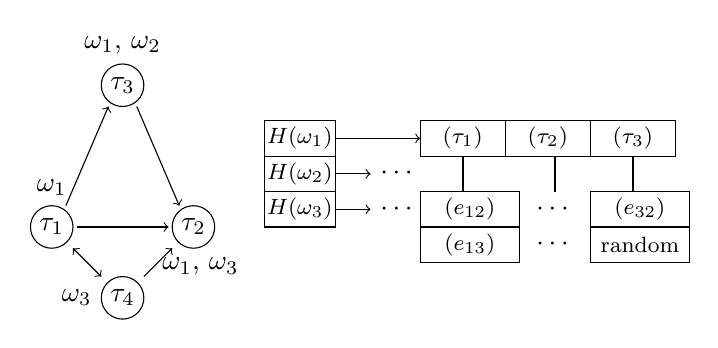
\begin{tikzpicture}[scale=.9]
\draw (0,0) circle (.3);
\node at (0,0) {$\tau_1$};
\node [above] at (0,.3) {$\omega_1$};
\draw (2,0) circle (.3);
\node at (2,0) {$\tau_2$};
\node [below] at (2.1,-.3) {$\omega_1$, $\omega_3$};
\draw (1,2) circle (.3);
\node at (1,2) {$\tau_3$};
\node [above] at (1,2.3) {$\omega_1$, $\omega_2$};
\draw (1,-1) circle(.3);
\node at (1,-1) {$\tau_4$};
\node [left] at (.7,-1) {$\omega_3$};
\draw [->] (.2,.3) -- (.8,1.7);
\draw [->] (1.2,1.7) -- (1.8,.3);
\draw [->] (.35,0) -- (1.65,0);
\draw [->] (1.3,-.7) -- (1.7,-.3);
\draw [<->] (.7,-.7) -- (.3,-.3);


\draw (3,0) rectangle (4,.5);
\node at (3.5,.25) {\footnotesize$H(\omega_3)$}; 
\draw [->] (4,.25) -- (4.5,.25);
\node [right] at (4.5,.25) {$\cdots$};
\draw (3,.5) rectangle (4,1);
\node at (3.5,.75) {\footnotesize$H(\omega_2)$};
\draw [->] (4,.75) -- (4.5,.75);
\node [right] at (4.5,.75) {$\cdots$}; 
\draw (3,1) rectangle (4,1.5);
\node at (3.5,1.25) {\footnotesize$H(\omega_1)$}; 
\draw [->] (4,1.25) -- (5.2,1.25);
\draw (5.2,1) rectangle (6.4,1.5);
\node at (5.8,1.25) {\footnotesize$\Enc(\tau_1)$};
\draw (6.4,1) rectangle (7.6,1.5);
\node at (7,1.25) {\footnotesize$\Enc(\tau_2)$};
\draw (7.6,1) rectangle (8.8,1.5);
\node at (8.2,1.25) {\footnotesize$\Enc(\tau_3)$};

\draw (5.2, 0) rectangle (6.6,.5);
\node at (5.9,.25) {\footnotesize$\Enc(e_{12})$};
\draw (5.2, -.5) rectangle (6.6,0);
\node at (5.9,-.25) {\footnotesize$\Enc(e_{13})$};
\draw (7.6, 0) rectangle (9, .5);
\node at (8.3,.25) {\footnotesize$\Enc(e_{32})$};
\draw (7.6, -.5) rectangle (9, 0);
\node at (8.3,-.25) {\footnotesize random};

\draw [thick](5.8, 1) -- (5.8,.5);
\draw [thick](7.1, 1) -- (7.1,.5);
\node at (7.1,.25) {$\cdots$};
\node at (7.1,-.25) {$\cdots$};
\draw [thick](8.2, 1) -- (8.2,.5);
\end{tikzpicture}
\caption{A small example of the delegating scheme. There are four documents $f_1$, $f_2$, $f_3$, $f_4$ (with tags $\tau_1$, $\tau_2$, $\tau_3$, $\tau_4$) and three keywords $\omega_1$, $\omega_2$, $\omega_3$. In the inverted list of $\omega_1$, there are three entries corresponding to the three documents which contain $\omega_1$. Among these three documents, there are three edges: from $\tau_1$ to both $\tau_2$ and $\tau_3$, and from $\tau_3$ to $\tau2$. Thus in the entry of $\Enc(\tau_1)$, we encrypt the edges $e_{12}$ and $e_{13}$; in the entry of $\Enc(\tau_3)$, we encrypt the edge $e_{32}$ (a random string is padded to hide the length information). The entry of $\Enc(\tau_2)$ encrypts no edge since $\tau_2$ has no out-edge among the three documents containing $\omega_1$. The entry of $\tau_2$ may be padded with some random strings for privacy. Clearly with $H(\omega_1)$ and $f_k(\omega_1)$, the cloud server can recover the subgraph of $\tau_1$, $\tau_2$ and $\tau_3$.}
\label{fig:gl}
\end{figure}

\subsection{Discussions}
One major improvement of the scheme above is that now the data owner does not need to compute the metric scores, which saves a lot of time in the Setup phase. The tremendous computation work is delegated to the cloud server, which usually has high computing speed and abundant hardware resource. Also the computation of metrics follows a \emph{lazy} pattern, i.e., they are computed only when needed. Since the distribution of queried keywords is usually highly biased, our improved scheme does not have to compute the metrics for all the documents or all the keywords in practice. Also it is clear that the improved scheme can be flexible to change network metric algorithms or policies, e.g., it is easy to change from PageRank to Betweenness Centrality.

Another important improvement is that we better support dynamic document insertion and deletion. Since each data structure is encrypted independently, the data owner can update them without refreshing the entire list.

\bibliographystyle{./IEEEtran}
\bibliography{./score_search}
\end{document}
